\section{Symulacja i weryfikacja}
\label{sec:sym-wer}

Błąd weryfikacji jest liczony jako suma kwadratów różnic między stanami osiągniętymi na koniec symulacji a tymi, które zostały podane jako wartości docelowe.

%-------------------------------------------------
\subsection{Przy użyciu pakietu JModelica.org}
\label{sub:sym-wer-jmodelica}

%TODO: opisać wpływ liczby elementów na rozwiązanie

%TODO: pokazać przykładowe wykresy

\subsubsection{Problemy z weryfikacją}
%TODO: opisać problemy z weryfikacją

\subsubsection{Problem dostępności interfejsu systemu Tango}

Biblioteka Tango Controls nakłada jeszcze jedno ograniczenie na część obliczeniową aplikacji: interfejs powinien być dostępny z maksymalnie trzysekundowym opóźnieniem. To znaczy, że każda prośba klienta musi zostać obsłużona w ciągu 3 sekund. W przypadku operacji symulacji, a szczególnie optymalizacji to założenie nie jest spełnione, ponieważ szczególnie ta druga operacja może trwać nawet kilka minut.

W API Tango Controls do języka Python (nazywającym się PyTango) istnieją sposoby na asynchroniczne wywoływanie operacji (tzw. \emph{green modes}), ale mają dwie wady:
\begin{itemize}
    \item używają tylko jednego wątku głównego aplikacji,
    \item procedury pakietu JModelica.org są z nimi niekompatybilne.
\end{itemize}

W związku z tym zaproponowano własne, ogólne rozwiązanie problemu potrzeby asynchronicznego wykonywania operacji wewnątrz klasy urządzeń. W tym celu użyto biblioteki \texttt{multiprocessing} wchodzącej w skład standardowego zestawu narzędzi języka Python. Za jej pomocą zaimplementowano asynchroniczne wywoływanie długich operacji w osobnych procesach, które po swoim końcu wywołuja metody odwołania (ang. \emph{callback}) w głównym wątku aplikacji. Dzięki temu wszystkie komendy, które wywołują długie operacje (\emph{Optimise}, \emph{RunSimulation} oraz \emph{RunVerification}) tylko uruchamiają osobny proces i przypisują odpowiednią metodę odwołania, nie blokując interfejsu urządzenia.

Osobnym procesem jest również serwer TCP. Posiada on własny system logowania i komunikuje się z głównym procesem aplikacji wyższego poziomu poprzez potok danych (ang. \emph{pipe}, nie mylić z częścią interfejsu urządzenia systemu Tango). Jest on dwukierunkowy: serwer może przez niego wysyłać aktualne dane odebrane od aplikacji niższego poziomu, a główny proces wszystkie informacje o sterowaniu. Odbiór danych po stronie serwera znajduje się na początku pętli obsługi komunikacji z klientem TCP (aplikacją niższego poziomu). Odbiór danych po stronie urządzenia odbywa się w odpytywanej co 50 milisekund komendzie \emph{GetDataFromDirectControl}.

Użyto w tym celu procesów, a nie wątków ze względu na tzw. \emph{Global Interpreter Lock} - globalny zamek interpretera. Jest to cecha języka Python, która powoduje, że wątki nie mogą być uruchamiane równolegle (nawet w przypadku dostępnych rdzeni procesora), a zawsze są tylko współbieżne. Z kolei procesy nie są objęte tym ograniczeniem i można ich używać w prawdziwie równoległy sposób.


%-------------------------------------------------
\subsection{Przy użyciu oprogramowania MATLAB/Simulink}
\label{sub:sym-wer-matlab}

%TODO: opisać okres próbkowania i inne ustawienia symulacji
%TODO: opisać wykresy i porównać z JModelicą

\begin{figure}
    \centering
    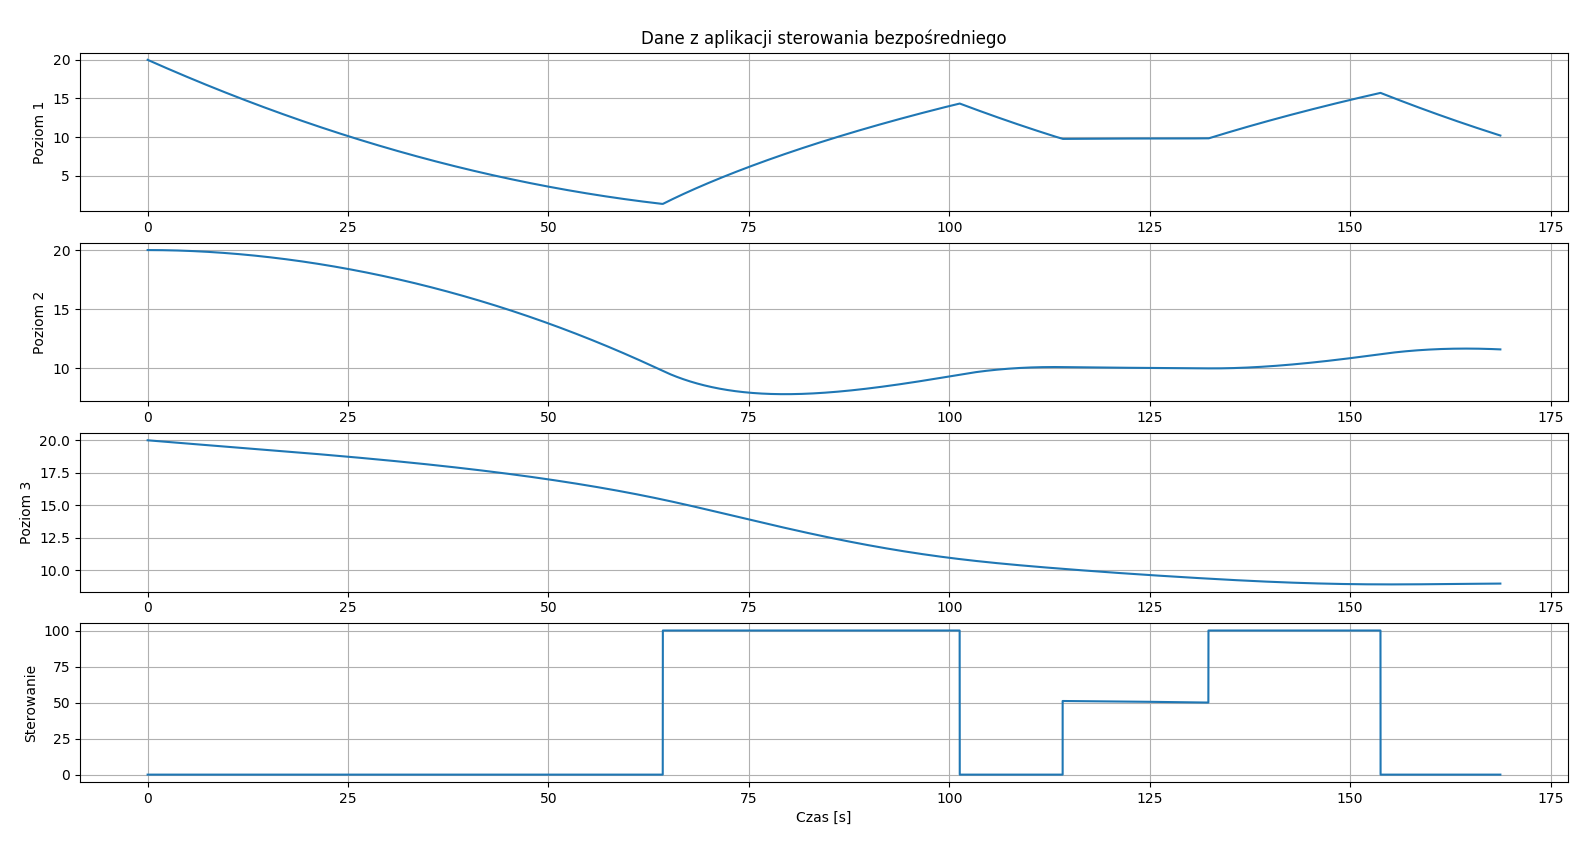
\includegraphics[scale=0.5,angle=90]{Grafika/ext_ctrl_2_opts}
    \caption{Dwa procesy optymalizacji zweryfikowane w symulacji niższym poziomem aplikacji. Źródło: własne.}
    \label{fig:extctrl2opts}
\end{figure}

\begin{figure}
    \centering
    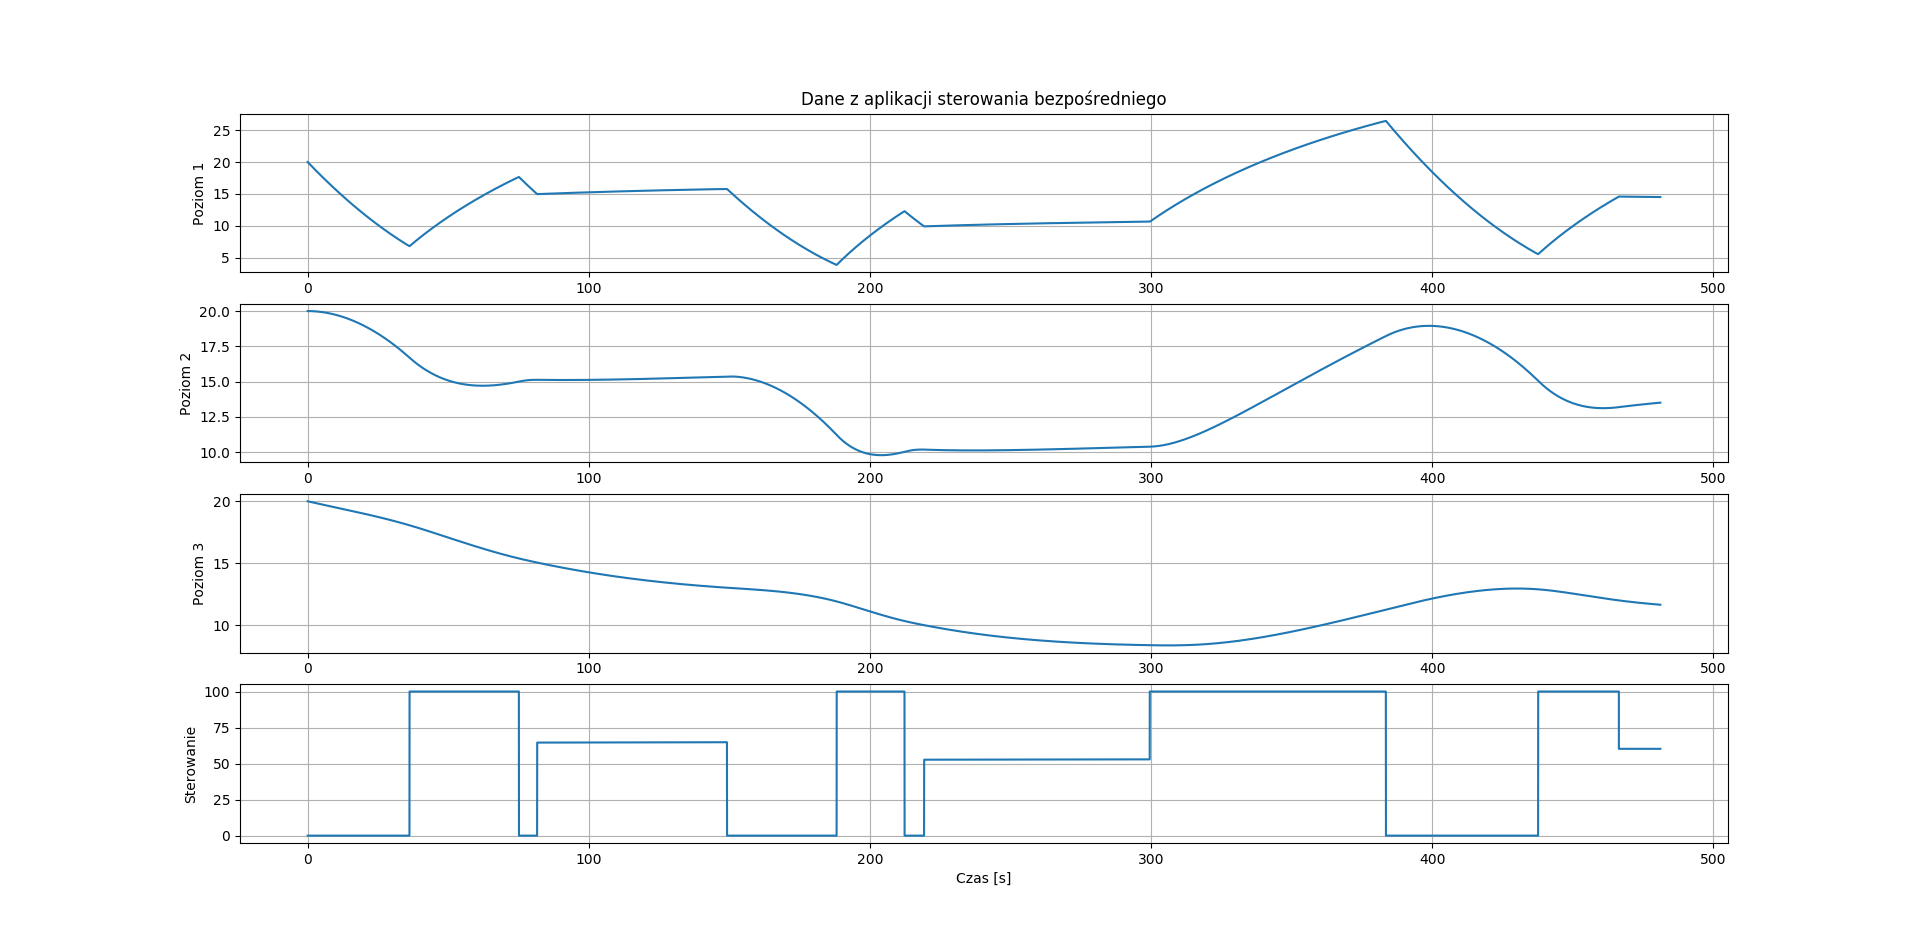
\includegraphics[scale=0.5,angle=90]{Grafika/ext_ctrl_3_opts}
    \caption{Trzy procesy optymalizacji zweryfikowane w symulacji niższego poziomu aplikacji. Źródło: własne.}
    \label{fig:extctrl3opts}
\end{figure}

